\documentclass[12pt,a4paper,titlepage]{article}
\usepackage[utf8]{inputenc}
\usepackage[german]{babel}
\usepackage{amsmath}
\usepackage{amsfonts}
\usepackage{amssymb}
\usepackage{setspace}
\usepackage{graphicx} %Um Bilder anzeigen zu können
\usepackage[top=1in, bottom=1.5in, left=1in, right=1in]{geometry}
\usepackage{endnotes}
\usepackage[section]{placeins}
\usepackage{fancyhdr}

\newcommand{\myma}{\fontfamily{pcr}\selectfont \textbf}
\newcommand{\mymo}{\fontfamily{pcr}\selectfont \textit}
\setlength{\parindent}{0pt}
\let\footnote=\endnote

\begin{document}
\pagestyle{fancy}

\begin{titlepage}
\vspace*{50pt}
\begin{center}
{\Huge Entwurf\\[1cm] {\bfseries Praxis der Softwareentwicklung}\\[2cm] Entwicklung einer Software zur Berechnung der Mandatsverteilung im Deutschen Bundestag\\[1cm]Gruppe 1} \\
\vspace*{15pt}
{\normalsize Philipp Löwer, Anton Mehlmann, Manuel Olk, Enes Ördek, \\Simon Schürg, Nick Vlasoff}
\end{center}
\date{}

\vspace*{30pt}
\begin{figure}[h]
\centering
		
\includegraphics[scale=0.6]{KIT-Logo.png}\\
		\vspace*{10pt}
		\Huge WS 2013 / 14
\end{figure}
\end{titlepage}
\newpage\thispagestyle{empty}\hspace{1em}\newpage
\def\Vhrulefill{\leavevmode\leaders\hrule height 0.7ex depth \dimexpr0.4pt-0.7ex\hfill\kern0pt}
\cfoot{{\Vhrulefill~  Seite \thepage   ~\Vhrulefill} \newline {\scriptsize KIT – Universität des Landes Baden-Württemberg und nationales Forschungszentrum in der Helmholtz-Gemeinschaft}}

\pagenumbering{roman} 

 
\newpage
\begin{onehalfspace}
\tableofcontents
\end{onehalfspace}
\newpage

\pagenumbering{arabic} 


\section{Einleitung}
Dieses Dokument beschreibt den Entwurf der im Pflichtenheft spezifizierten Software zur Berechnung der Mandatsverteilung im Deutschen Bundestag.\\
Anhand verschiedener Diagramme, im speziellen einem Klassendiagramm, werden die Architektur, die Komponenten, die Module und die einzelnen Klassen inklusive ihrer Schnittstellen und ihrer Attribute erläutert.\\
Desweiteren werden Entwurfsentscheidungen, Entwurfsdetails und die verwendeten Entwurfsmuster erläutert sowie zentrale Abläufe im Programm mit Hilfe von Sequenzdiagrammen visualisiert.\\
Abschließend wird die Zeitplanung der Implementierung und die zugehörigen Hauptverantwortlichen in einem Gantt-Diagramm dargestellt.    

\section{Systemmodell}
\section{Klassendiagramm}
\subsection{GUI}
\begin{figure}[!ht]
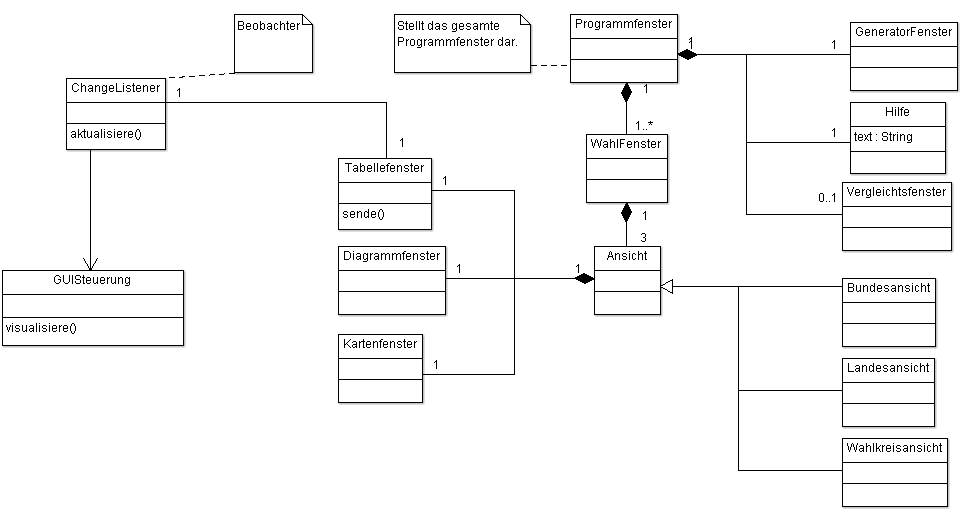
\includegraphics[scale=0.4]{GUI-Abschnitt.png} \caption{GUI Komponente} 
\end{figure}

Dieser Teil des gesamten Klassendiagramm zeigt den Visualisierungsteil. \\
Das {\myma{Programmfenster}} besteht aus einem oder mehreren {\myma{Wahlfenstern}} in Form von Tabs. Weiterhin enthält es
ein {\myma{Generatorfenster}}, um nicht identifizierten Parteien Stimmen zu geben, die Hilfe, und
ein Vergleichsfenster, wenn der Vergleich zweier Wahlen aktiv ist. \\
Ein Wahlfenster hat eine bestimmte Ansicht, diese ist entweder die Bundes-, Landes- und
Wahlkreisansicht. Zu jeder von diesen gehört jeweils ein Tabellen-, Diagramm- und Kartenfenster. \\
Das Tabellenfenster zeigt die Daten der Bundestagswahl-Klasse an (Erst-, Zweitstimmen, Direktmandat,...).\\
Das Diagrammfenster visualisiert die Sitzverteilungs-Klasse. \\
Das Kartenfenster visualisiert die Deutschland-Klasse. \\
Das Tabellenfenster, in welchem Erst- und Zweitstimmen geändert werden können, und die
dazugehörige ChangeListener-Klasse werden im Beobachter-Prinzip umgesetzt. Der ChangeListener
hört das Tabellenfenster ab und wird bei Veränderungen informiert. \\
Gesteuert werden alle genannten Klassen durch die GUISteuerungs-Klasse, die die Ansicht und das
Vergleichsfenster visualisiert und das gesamte Programmfenster beim Programmstart initialisiert.


\begin{large}
Methoden 
\end{large}
\begin{description}
\item \textbf {Tabellenfenster} \\
\begin{itemize}
\item \textbf {senden(aenderungszeile : String, wert : Integer)} \\
Das Tabellenfenster informiert den ChangeListener darüber, welche Zeile im Tabellenfenster
geändert  wurde und was der neue Wert ist. \\
\end{itemize}
\item \textbf {ChangeListener} \\
\begin{itemize}
\item \textbf {aktualisiere()} \\
Der ChangeListener passt seine Attribute, nachdem er von dem Tabellenfenster informiert wurde, an,
diese repräsentieren den zuletzt geänderte Tabelleneintrag. \\
\item \textbf {uebergeben()} \\
Der ChangeListener übergibt, nachdem seine Attribute neu gesetzt wurden, diese an die Steuerung,
sich dann um die Aktualisierung der internen Daten kümmert. \\
\end{itemize} 
\item \textbf {GUISteuerung} \\
\begin{itemize}
\item \textbf {initialisiere()} \\
Der Programmfensterkonstruktor wird aufgerufen, alle Objekte erstellt und mit der Wahl 2013 befüllt. \\
\item \textbf {visualisiere(bw : Bundestagswahl)} \\
Wurde eine neue Bundestagswahl geladen und berechnet, werden alle dazugehörigen Werte und Grafiken
im Karten-, Diagramm- und Tabellenfenster geladen. \\ 
\item \textbf {visualisiere(vergleich : Vergleich)} \\
Hat die Steuerung einen Vergleich zweier Wahlen errechnet und die Daten an die GUISteuerung übergeben,
wird das Vergleichsfenster erstellt und mit den Daten des Vergleichsobjektes gefüllt. \\
\item \textbf {zurueckSetzen(bw : Bundestagswahl)} \\
Wünscht der Benutzer einen zuvor geänderten Wert im Tabellenfenster zurückzusetzen, wird die Steuerung 
informiert. \\
\end{itemize}

\end{description}
\newpage
\subsection{Datenhaltung}
\begin{figure}[!ht]
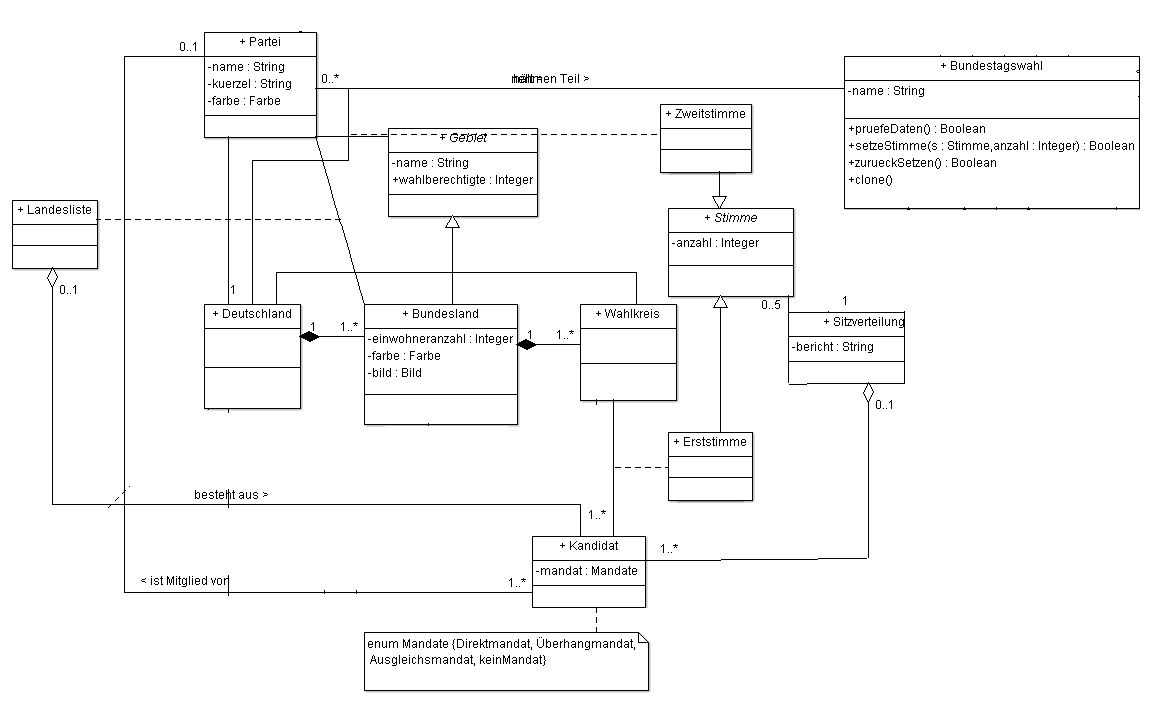
\includegraphics[scale=0.4]{Datenhaltung-Ausschnitt} \caption{Datenhaltungs Komponente} 
\end{figure}

Dieser Ausschnitt des Klassendiagramms stellt den Datenhaltungsteil dar.
\newpage
\subsection{Import/ Export}
\begin{figure}[!ht]
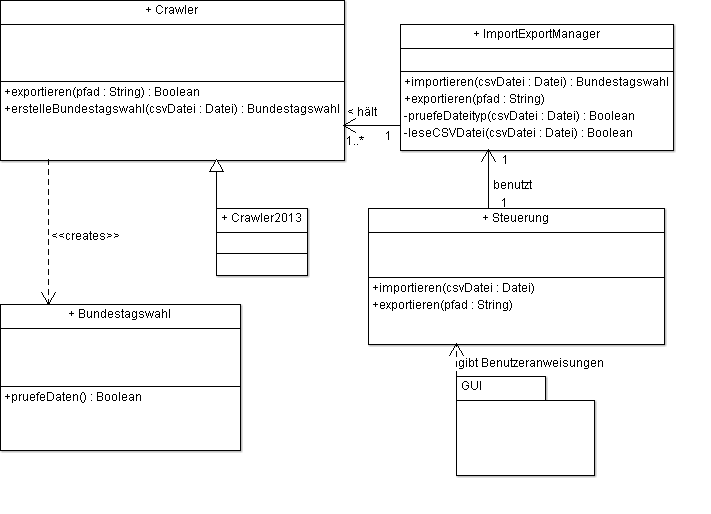
\includegraphics[scale=0.5]{Import-Export_Ausschnitt} \caption{Import/Export Komponente} 
\end{figure}

Hier sieht man den Aufbau des Import- bzw. Exportmoduls. Zur Übersichtlichkeit werden die zum Importieren/Exportieren nicht notwendigen Methoden in {\myma{Steuerung}} und die genaue Struktur hinter {\myma{Bundestagswahl}} und der GUI ausgeblendet. \\
Mit dem Programm wird nur ein vorimplementierter Crawler mitgegeben, der .csv-Dateien, die dem Format der .csv-Datei zur Bundestagswahl 2013 der Bundeswahlleiter-Webseite entsprechen, auswerten kann - dies ist {\myma{Crawler2013}}. Um jedoch die Möglichkeit zu garantieren, nachträglich weitere Crawler hinzuzufügen, haben wir uns dafür entschieden, eine abstrakte Oberklasse {\myma{Crawler}} zu verwenden, von der {\myma{Crawler2013}} erbt, und alle vorhandenen Crawler von der Klasse {\myma{ImportExportManager}} halten zu lassen. \\ Ausgelöst wird der ganze Import- bzw. Exportvorgang durch eine Benutzerinteraktion (z.B. Betätigen des Laden- Knopfs im Menü), worauf {\myma{Steuerung}} die entsprechenden Methoden von {\myma{ImportExportManager}} ausführt.

\subparagraph{Methoden}
\begin{description}
\item{\myma{ImportExportManager}}
\item {\mymo{importieren(csvDatei : Datei) : Bundestagswahl}} \\
Diese öffentliche Methode führt zuerst die private Methode {\mymo{pruefeDateityp(csvDatei : Datei) : Boolean}} aus. Wenn diese true zurückgibt, wird die ebenfalls private Methode {\mymo{leseCSVDatei(csvDatei : String) : Boolean}} ausgeführt. Wurde nun eine gültige Bundestagswahl zurückgegeben, wird diese an die Steuerung zurückgegeben, andernfalls ein Fehler ausgegeben.

\item {\mymo{exportieren(pfad : String)}} \\


\item {\mymo{pruefeDateityp(csvDatei : Datei) : Boolean}} \\
Prüft, ob es sich bei der gegebenen Datei um eine .csv-Datei handelt. Wenn dies der Fall ist, wird true zurückgegeben, andernfalls false.

\item {\mymo{leseCSVDatei(csvDatei : String) : Boolean}} \\
Durchläuft die Crawler-Liste und lässt die darin enthaltenen Crawler nacheinander versuchen, die .csv-Datei auszuwerten und mit den gewonnen Informationen eine Bundestagswahl zu erstellen und zu füllen. Gelingt es einem Crawler, wird der Durchlauf abgebrochen und die gerade erstellte Bundestagswahl wird an den ImportExportManager zurückgegeben.
\end{description}

\subsection{Wahlgenerierung}
\begin{figure}[!ht]
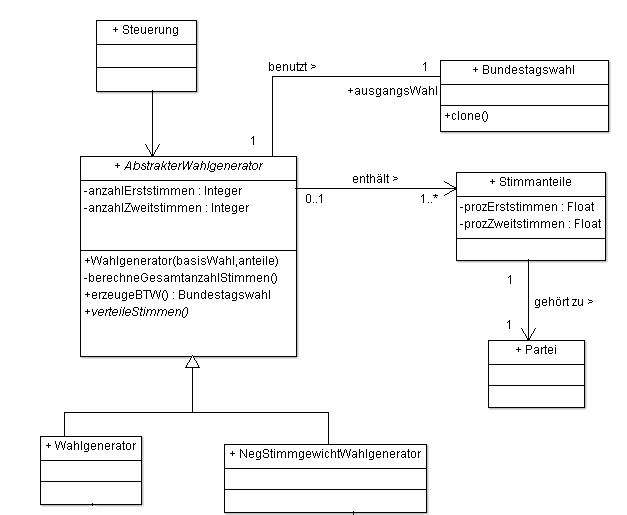
\includegraphics[scale=1.0]{Klassendiagramme/Wahlgenerator_Klassendiagramm.png} \caption{Wahlgenerierungs-Komponente} 
\end{figure}
\newpage
Der obige Ausschnitt des Klassendiagramms zeigt das Wahldatengenerierungs-Modul.\\\\
Zur Übersichtlichkeit werden in den Klassen {\myma{Partei}}, {\myma{Steuerung}} und {\myma{Bundestagswahl}} nur die für dieses Modul relevanten Informationen angezeigt.\\\\
Mit diesem Modul können {\myma{Bundestagswahl}} Objekte anhand vorher definierten {\myma{Stimmanteilen}} auf Bundesebene generiert werden. Bei {\myma{Stimmanteile}} handelt es sich um eine Liste aller Parteien mit prozentualen Anteilen der Erst- und Zweitstimmen auf Bundesebene. Des weiteren benötigt der Wahlgenerator eine {\myma{basisWahl Bundestagswahl}} um Daten wie beispielsweise {\myma{Bundesländer}}, {\myma{Wahlkreise}} und {\myma{Wahlberechtigte}} zur Verfügung zu haben. Aus dieser basisWahl wird eine tiefe Kopie erstellt, deren Stimmzahlen anschließend verändert werden.\\\\

Neben dem {\mymo Wahlgenerator}, der alle Stimmen der jeweiligen Parteien zufällig auf Wahlkreise verteilt gibt es noch den {\mymo NegStimmgewichtWahlgenerator}. Dieser erzeugt Bundestagswahlen, die die Voraussetzungen erfüllen, welche für die Simulation des Negativen Stimmgewichts benötigt werden.

\subparagraph{Methoden}
\begin{description}
\item {\mymo{Wahlgenerator(basisWahl : Bundestagswahl, anteile : Stimmanteile)}} \\
Der Konstruktor dieser Klasse. Wird verwendet um einen neuen {\mymo{Wahlgenerator}} zu erstellen. Hier werden die Attribute basisWahl, anteile, erststimmenAnzahl und zweitstimmenAnzahl gesetzt.
\item {\mymo{berechneGesamtanzahlStimmen()}} \\
Diese Methode ist privat und wird von dem Konstruktor verwendet um die Attribute {\mymo{anzahlErststimmen}} und {\mymo{anzahlZweitstimmen}} zu berechen. Hierzu werden die Stimmanteile mithilfe der Anzahl aller Wahlberechtigten in absolute Zahlen für Erst- und Zweitstimmen umgerechnet.
\item {\mymo{erzeugeBTW() : Bundestagswahl}} \\
Erzeugt eine neue Bundestagswahl auf der Grundlage der basisWahl und füllt diese mit den Erst- und Zweitstimmen.
\item {\mymo{verteileStimmen()}} \\
Diese Methode verteilt alle Erst- und Zweitstimmen auf die Wahlkreise der Bundestagswahl. Diese Methode muss in jeder Unterklasse von Wahlgenerator implementiert werden.
\end{description}

\newpage
\subsection{Chronik}
\begin{figure}[!ht]
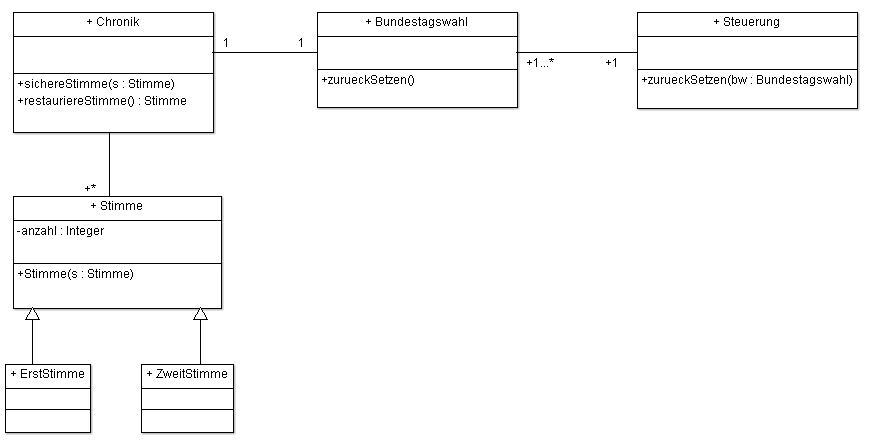
\includegraphics[scale=0.8]{Chronik_Ausschnitt} \caption{Chronik-Komponente} 
\end{figure}

Die Klasse {\myma{Chronik}} gibt dem Programm die Funktionalität, Veränderungen an den Stimmen rückgängig zu machen. Jede {\myma{Bundestagswahl}} hat hierbei eine eigene Chronik. {\myma{Chronik}} wird in dem Konstruktor von {\myma{Bundestagswahl}} erzeugt, und ist daher in jedem {\myma{Bundestagswahl}}-Objekt enthalten. Es besitzt eine Menge von {\myma{Stimmen}}-Objekten. Bei jeder Veränderung wird ein neues {\myma{Stimmen}}-Objekt angelegt, was die Veränderung wiederspiegelt.
\
Die Methode {\myma{sichereStimme}} wird von dem {\myma{Bundestagswahl}}-Objekt bei jedem Aufruf von {\myma{setzeStimme}} aufgerufen.
\subparagraph{Methoden}
\begin{description}
\item {\mymo{sichereStimme(s : Stimme)}} \\
Diese Funktion wird von dem assoziierten {\myma{Bundestagswahl}}-Objekt innerhalb der {\mymo{setzeStimme}}-Funktion aufgerufen. Falls bereits fünf {\myma{Stimmen}}-Objekte vorhanden sind, wird das älteste entfernt.
\item {\mymo{restauriereStimme() : Stimme}} \\
Wird von der {\myma{Steuerung}} über die aktuelle Bundestagswahl mit der Funktion{\mymo{zurueckSetzen()}} aufgerufen und gibt die zuletzt hinzugefügte {\myma{Stimme}} zurück. Die Bundestagswahl ersetzt dann die aktuelle Stimme mit der restaurierten Stimme.
\end{description}

\newpage
\subsection{Mandatsrechner}
\begin{figure}[!ht]
\centering
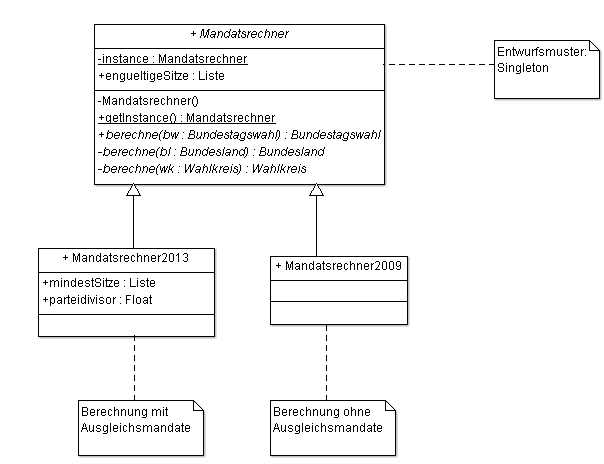
\includegraphics[scale=0.6]{Mandatsrechneralles.png} \caption{Mandatsrechner-Komponente} 
\end{figure}
Die Berechnung der Wahl wird mit Hilfe des {\myma{Mandatsrechners}} realisiert. Es stehen die Klasse \\{\myma{Mandatsrechner2013}}, die das Berechnungsverfahren von der Bundestagswahl 2013 benutzt und die Klasse {\myma{Mandatsrechner2009}}, die das Berechnungsverfahren von der Bundestagswahl 2009 benutzt zur Verfügung. Beide Klassen erben von der abstrakten Klasse {\myma{Mandatsrechner}}. Dadurch besteht die Möglichkeit, weitere Berechnungsverfahren in späteren Versionen zu dem Programm hinzuzufügen. Da nur ein Objekt von dem {\myma{Mandatsrechner}} gebraucht wird, wird das Entwurfsmuster Einzelstück eingesetzt. Deswegen hält die Klasse einen privaten Konstruktor. Die abstrakten Methoden {\mymo{berechne()}} werden überladen, damit sie durch ihre Eingabeparameter spezifiziert werden. Diese werden dann in den Unterklassen je nach Wahlgesetz angepasst. Neben der Berechnung wird ein Bericht über die Sitzverteilung erstellt, der zum Nachvollziehen der Sitzverteilung helfen soll.
\begin{large}
Methoden 
\end{large}
\begin{description}

\item {\mymo{berechne(wk: Wahlkreis):Wahlkreis}} \\
Es werden die Stimmen aus den jeweiligen Wahlkreis ausgewertet. Dabei wird der Wahlkreissieger bestimmt und die Anzahl der Zweitstimme von jeder Partei. Die Auswertung wird danach wieder in das Wahlkreis-Objekt geschrieben.
\item {\mymo{berechne(bl: Bundesland):Bundesland}} \\
Um das Bundesland zu berechnen, müssen vorher alle Wahlkreise berechnet werden. Deswegen werden alle Wahlkreise, die ein Bundesland hält, neu berechnet. Die Berechnung der einzelnen Bundesländer erfolgt parallel. Nachdem die berechneten Wahlkreise im Bundesland gespeichert wurden, wird das Bundesland berechnet. Hier wird das Verhältnis der Parteien im Bundesland berechnet, damit später klar ist wie viele Sitze eine Partei in diesem Bundesland bekommt. Diese Ergebnisse werden, wie beim Wahlkreis, im Bundeslandobjekt gespeichert und danach zurückgegeben. 
\item {\mymo{berechne(bw: Bundestagswahl):Bundestagswahl}} \\
Diese öffentliche Methode berechnet zuerst alle Bundesländer die sich in der Klasse befinden. Nachdem alle Bundesländer erfolgreich berechnet wurden, wird die endgültige Sitzverteilung nach dem jeweiligen Wahlgesetz berechnet. Die Sitzverteilung wird dann in dem Bundestagswahlobjekt gespeichert. Das Bundestagswahlobjekt wird danach wieder an die Steuerung zurückgegeben.
\item {\mymo{erstelleBericht(Zeile : String)}} \\
Während der Berechnung wird nebenbei eine Sitzverteilungsbericht verfasst, der beschreiben soll, wie die Sitzverteilung entstanden ist. Dabei wird die Methode immer aufgerufen, wenn eine Partei einen Sitz in der Sitzverteilung bekommen hat. Dies wird dann mit einer Zeile im Bericht protokolliert.
\end{description} 

\subsection{Meldung}
\begin{figure}[!ht]
\centering
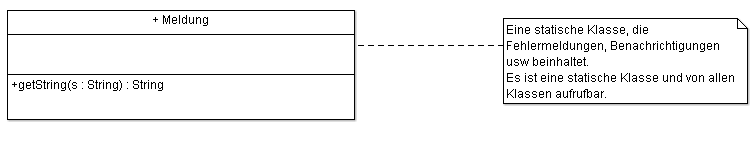
\includegraphics[scale=0.8]{Meldung_Ausschnitt.png} \caption{Meldungs-Klasse} 
\end{figure}
Die Klasse {\myma{Meldung}} ist verantwortlich für Fehlermeldungen, Benachrichtigungen und Fenstertexte. Es ist eine statische Klasse. Die Funktion {\mymo{getString}} gibt zu einem gegebenen Schlüssel ein String zurück. Die Strings dieser Klasse werden in einem externen Textdokument gelagert.


\section{Anwendungsfälle}



\section{Sequenzdiagramme}
\subsection{Import}
\begin{figure}[!ht]
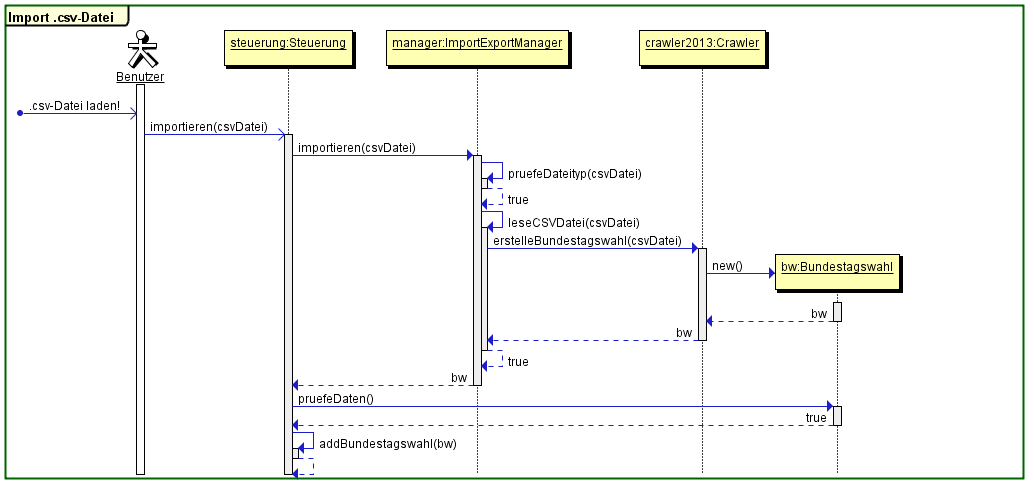
\includegraphics[scale=0.5]{Sequenzdiagramme/Import_Sequenzdiagramm.png} \caption{Import Sequenzdiagramm} 
\end{figure}


\subsection{Wahlgenerierung}
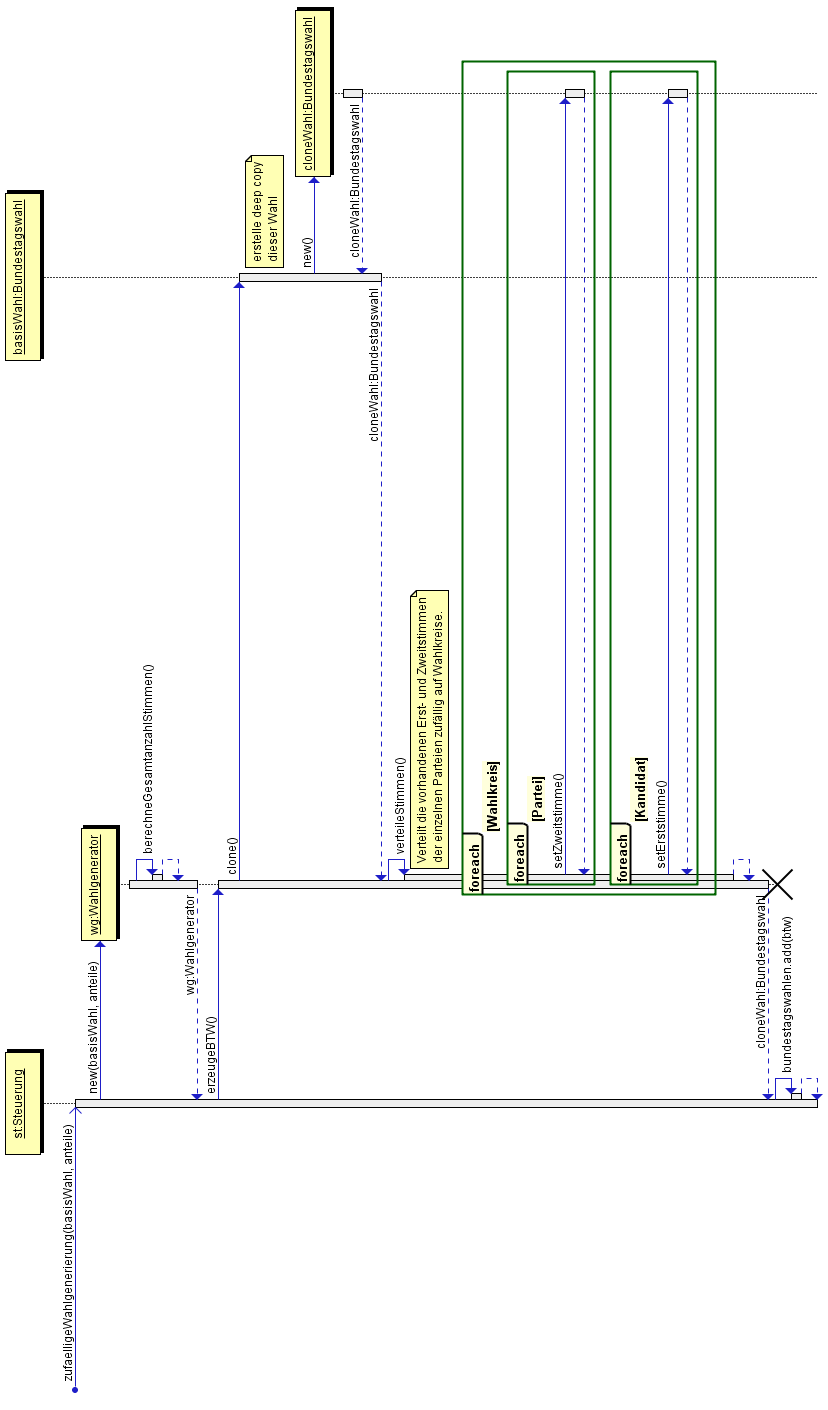
\includegraphics[scale=0.45]{Sequenzdiagramme/Wahlgenerierung.png}
Beim Generieren einer Bundestagswahl werden die Stimmanteile mithilfe der Anzahl aller Wahlberechtigten in absolute Zahlen für Erst- und Zweitstimmen umgerechnet. Diese Stimmen werden dann zufällig auf die einzelnen Wahlkreise verteilt.\\\\
Dieser Vorgang ist im folgenden noch einmal als Sequenzdiagramm aufgezeigt.
Neben der zufälligen Verteilung von den Stimmen auf alle Bundesländer und Wahlkreise gibt es noch einen Wahlgenerator der Stimmverteilungen erzeugt, die nach dem Wahlgesetz von 2009 zu negativem Stimmgewicht durch Überhangsmandate führen. Diese werden benötigt um in einer Vergleichsansicht das negative Stimmgewicht zu verdeutlichen.
\subsection{Paradoxe Wahlgenerierung und Vergleich}

\subsection{Vergleich}

\subsection{Chronik}
\begin{itemize}
	\item Veränderung an den Stimmen \\
		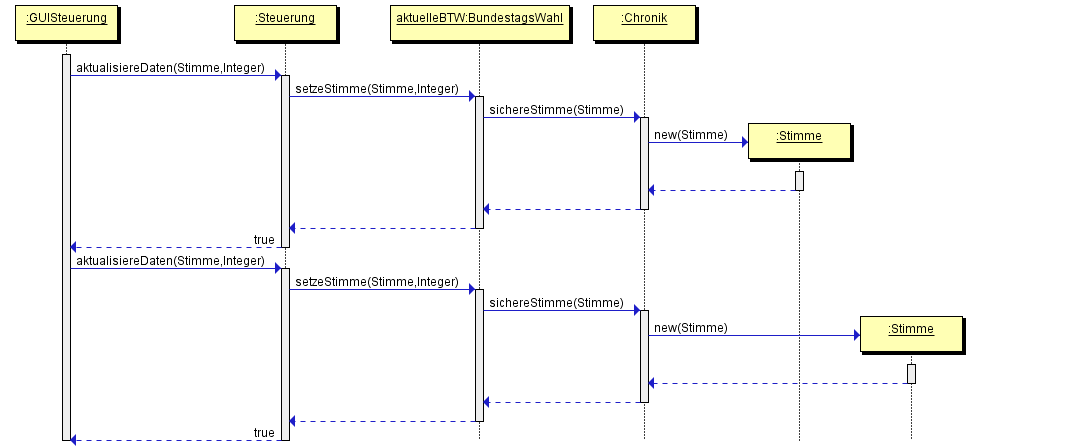
\includegraphics[scale=0.7]{Chronik_Sequenzdiagramm-stimmenaendern.png}
	\item Restaurieren einer Stimme \\
		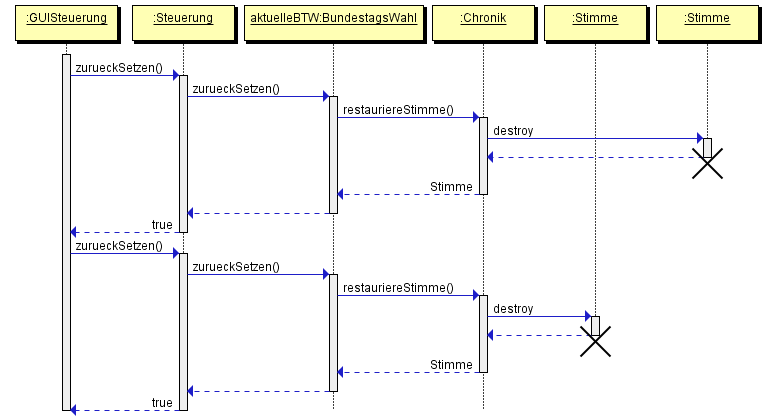
\includegraphics[scale=0.7]{Chronik_Sequenzdiagramm-restaurieren.png}
		\\
		Stimmen werden in der Chronik werden Stack-artig zurückgegeben. Sobald eine Bundestagswahl rückgängig gemacht wurde, wird die neue Bundestagswahl als Rückgabewert zurückgegeben.
	\item Beispielszenario	
\end{itemize}
%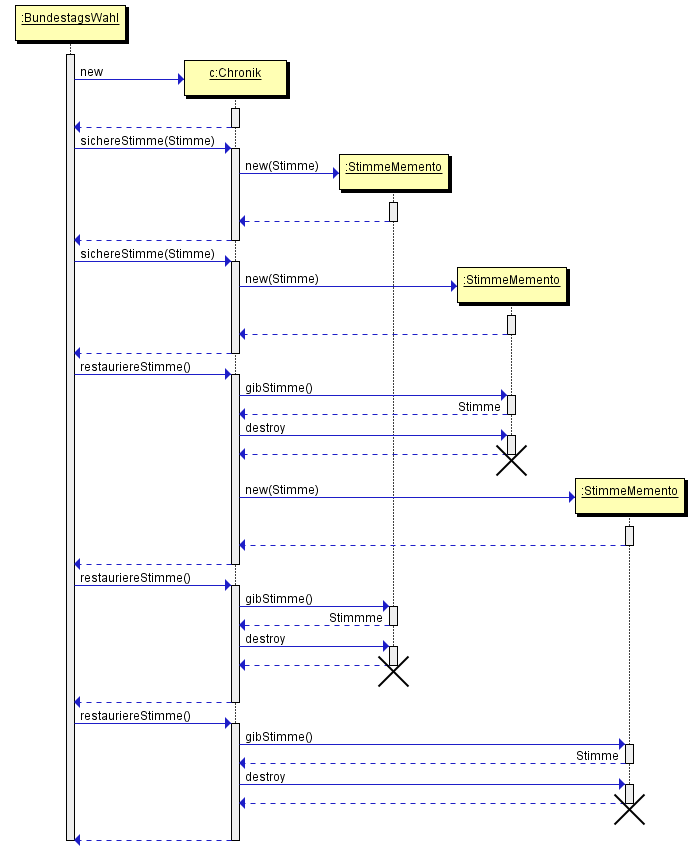
\includegraphics[scale=0.75]{Chronik_Sequenzdiagramm.png}

\begingroup
\parindent 0pt
\parskip 2ex
\def\enotesize{\normalsize}

\endgroup
\end{document}
